\chapter{Resultados}

\section{Resultados cuantitativos}
La Figura~\ref{fig:fidelity-means} muestra las medias por condición. Tanto EDSR como SwinIR
superaron a la interpolación bicúbica en PSNR-Y y SSIM-Y en las seis condiciones; los 24 intervalos
correspondientes ---dos métodos aprendidos, dos métricas y seis condiciones--- quedaron por encima
de cero. La magnitud, sin embargo, dependió claramente de la degradación. En \texttt{x2-clean},
EDSR mejoró a bicúbica en 4,345 dB y 0,0595 SSIM, mientras que SwinIR alcanzó 5,670 dB y 0,0695.
En \texttt{x2-strong} las ventajas se redujeron a 0,199 dB y 0,0074 para EDSR, y 0,176 dB y
0,0043 para SwinIR. Que los intervalos excluyan cero no convierte estos últimos efectos en una
mejora profesional relevante.

\begin{figure}[htbp]
  \centering
  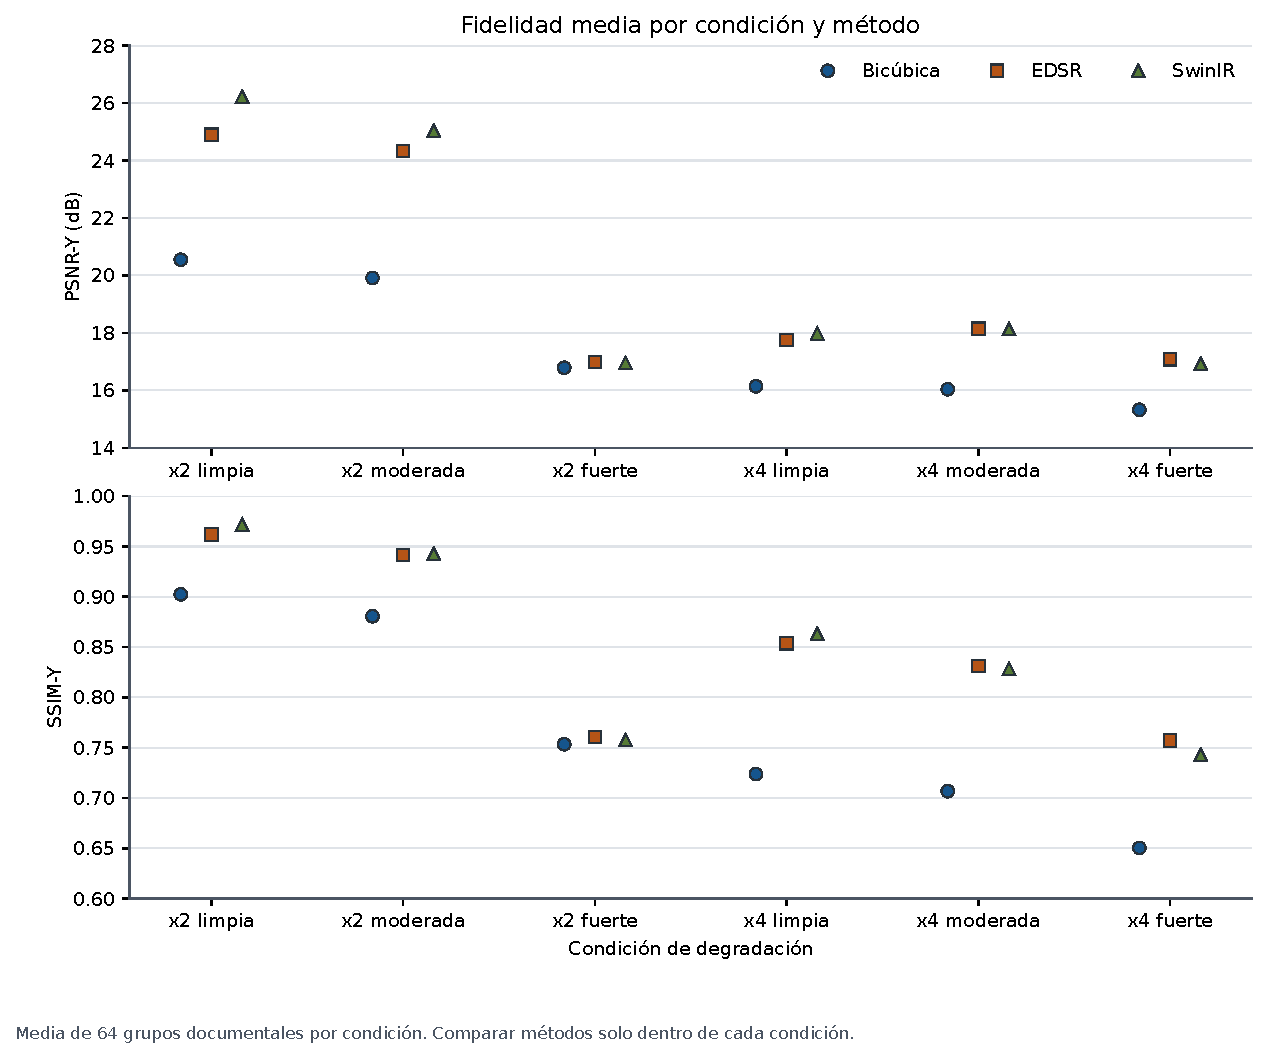
\includegraphics[width=\textwidth]{figures/results/fidelity-means.pdf}
  \caption{PSNR-Y y SSIM-Y medios para los 64 grupos documentales en cada condición. Las
  comparaciones solo son válidas dentro de la misma escala y perfil. Fuente: elaboración propia a
  partir del experimento SMB v2.}
  \label{fig:fidelity-means}
\end{figure}

La comparación directa entre las dos redes evita declarar un ganador por sus medias aisladas
(Tabla~\ref{tab:swinir-edsr}). Los intervalos favorecieron a SwinIR en las dos métricas para
\texttt{x2-clean}, \texttt{x2-moderate} y \texttt{x4-clean}. En \texttt{x2-strong} y
\texttt{x4-moderate}, el intervalo de PSNR cruzó cero y SSIM favoreció a EDSR. En
\texttt{x4-strong}, EDSR fue superior en ambas medidas. Por tanto, la mayor complejidad del
transformador no produjo una ventaja general.

\begin{table}[htbp]
  \centering
  \small
  \caption{Diferencia media emparejada SwinIR menos EDSR e intervalo percentil del 95\,\% por
  fuente. Un intervalo que cruza cero se marca como no resuelto. Fuente: elaboración propia.}
  \label{tab:swinir-edsr}
  \begin{tabular}{lrr}
    \toprule
    Condición & \(\Delta\) PSNR-Y (dB) & \(\Delta\) SSIM-Y \\
    \midrule
    x2 limpia    &  1,325 [1,178; 1,480]  &  0,0100 [0,0092; 0,0109] \\
    x2 moderada  &  0,704 [0,574; 0,835]  &  0,0014 [0,0002; 0,0024] \\
    x2 fuerte    & -0,023 [-0,074; 0,020] & -0,0031 [-0,0050; -0,0015] \\
    x4 limpia    &  0,230 [0,137; 0,336]  &  0,0094 [0,0074; 0,0116] \\
    x4 moderada  & -0,011 [-0,054; 0,033] & -0,0029 [-0,0042; -0,0015] \\
    x4 fuerte    & -0,152 [-0,197; -0,107]& -0,0142 [-0,0165; -0,0117] \\
    \bottomrule
  \end{tabular}
\end{table}

La Figura~\ref{fig:paired-deltas} completa esta lectura mostrando las ganancias de cada red frente
a la referencia bicúbica con su incertidumbre emparejada. Los resultados negativos y las
comparaciones no resueltas se conservaron en el análisis y no se sustituyeron por una selección de
condiciones favorables.

\begin{figure}[htbp]
  \centering
  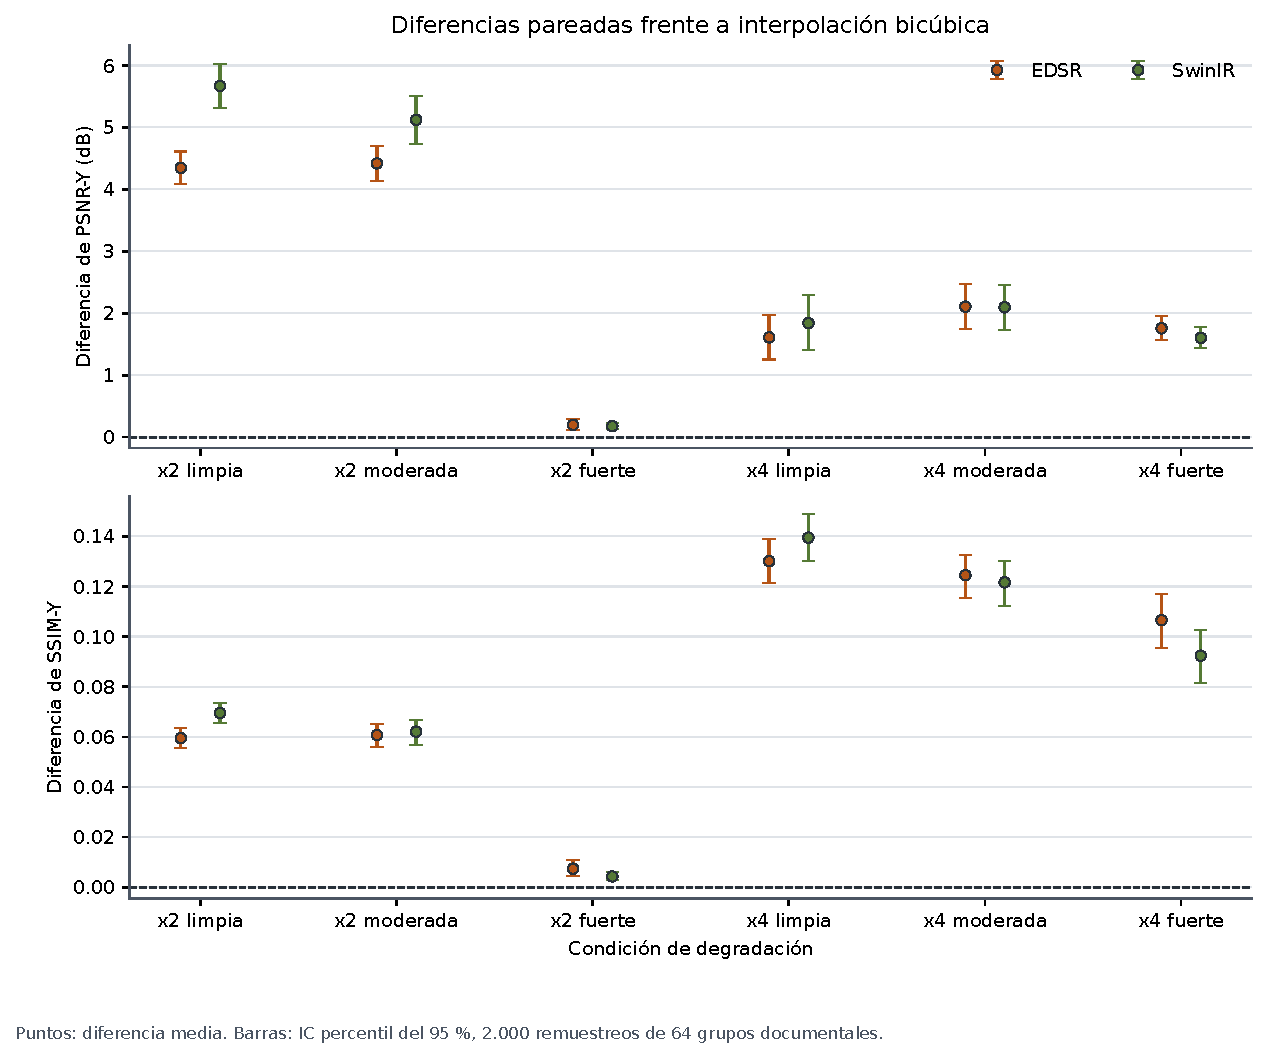
\includegraphics[width=\textwidth]{figures/results/paired-deltas-vs-bicubic.pdf}
  \caption{Ganancia media emparejada de EDSR y SwinIR respecto a bicúbica, con intervalos del
  95\,\% obtenidos al remuestrear las 64 fuentes. Fuente: elaboración propia.}
  \label{fig:paired-deltas}
\end{figure}

\section{Resultados cualitativos y fallos musicales}
La lectura visual sigue la secuencia referencia HR, entrada LR y salidas de los modelos.
La página completa permite comprobar disposición y legibilidad globales; las ampliaciones
muestran separaciones, contornos y signos que se pierden al reducir la página para imprimirla.
En cada comparación se utiliza exactamente la misma región y el mismo tamaño de visualización.
Cada caso de detalle ocupa una página propia, con dos columnas, para que los símbolos se puedan
examinar a mayor tamaño. Las imágenes se incrustan en PDF a su resolución nativa, sin reducción
previa de píxeles ni compresión con pérdidas. Las vistas de página completa aportan contexto;
el juicio sobre trazos finos se apoya en las ampliaciones y en el zoom del documento digital.
La LR se amplía por vecino más próximo, sin suavizado añadido. Los casos pertenecen a la revisión
cualitativa fijada; los recortes se eligieron después para explicar sus observaciones, no para
recalcular valoraciones ni para estimar la frecuencia de un defecto.

En las 18 valoraciones fijas se registró \emph{sin incidencia clara} en cuatro de los seis casos
bicúbicos y en dos de los seis casos de cada red. Se observaron incidencias en dos casos bicúbicos,
cuatro EDSR y cuatro SwinIR. Estos recuentos describen únicamente las seis páginas fijadas y no son
tasas de error ni permiten ordenar métodos por seguridad.

Los tres métodos quedaron sin incidencias claras en las condiciones x2 limpia y x2 moderada. En el
caso x2 fuerte, la entrada seguía siendo legible y bicúbica no
añadió un defecto claro, pero tampoco produjo una mejora apreciable; EDSR y SwinIR perdieron detalle
en símbolos y añadieron textura o \emph{ringing}. En los casos \(\times 4\) aparecieron
simplificación de símbolos, corrupción de texto o dígitos y reconstrucción de líneas rectas como
trazos ligeramente curvos. En \texttt{x4-moderate}, SwinIR reconstruyó visualmente las notas mejor
que EDSR en el caso revisado, pese a mantener defectos en otros símbolos o dígitos. En x4 fuerte,
parte del daño procedía ya de la degradación y ninguno de los tres métodos lo
recuperó de manera fiable.

La Figura~\ref{fig:pretrained-qualitative} hace visible esa discrepancia entre una puntuación
global y la lectura localizada. En el caso fijo \texttt{smb-test-000210}, EDSR y SwinIR obtuvieron
valores prácticamente empatados ---18,314 y 18,311 dB de PSNR-Y; 0,7960 y 0,7932 de SSIM-Y---,
por encima de la bicúbica ---15,949 dB y 0,6696---. Sin embargo, el recorte revela que la valoración
no depende solo de nitidez: las redes recuperan mejor las notas que la interpolación, pero alteran
textura, dígitos y geometría fina; en esta región, el revisor consideró más reconocibles las notas
de SwinIR que las de EDSR. La referencia HR impide confundir una salida más contrastada con una
reconstrucción necesariamente correcta.

\begin{figure}[htbp]
  \centering
  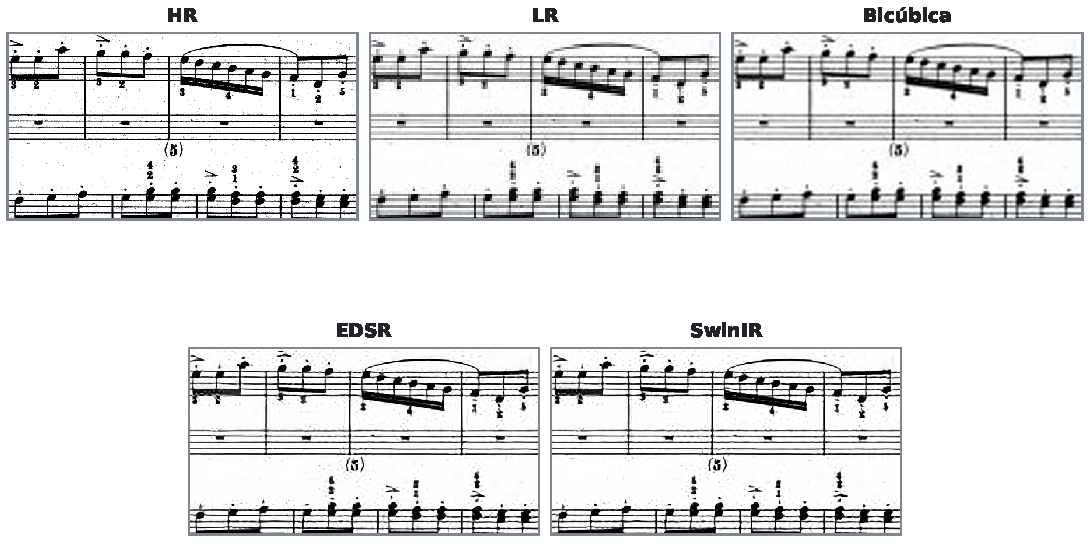
\includegraphics[width=\textwidth]{figures/results/pretrained-comparison-x4-moderate.pdf}
  \caption[Comparación cualitativa de los métodos preentrenados]{Referencia, entrada LR y salidas
  de los tres comparadores para el caso fijo \texttt{smb-test-000210} bajo
  \texttt{x4-moderate}. La LR se amplía por vecino más próximo. El ejemplo conserva tanto la
  mejora sobre bicúbica como los defectos que impiden declarar un ganador solo por PSNR-Y o
  SSIM-Y. Fragmento de la Sonata L.55/K.330 de Domenico Scarlatti, identificada como
  \texttt{scarlatti\_l055k330}. Fuente: elaboración propia a partir de SMB
  \cite{smbDatasetCard}.}
  \label{fig:pretrained-qualitative}
\end{figure}

La Figura~\ref{fig:pretrained-details} reúne tres situaciones distintas del muestreo fijo.
En A, la entrada x2 limpia conserva la estructura y las redes definen los trazos sin una incidencia
clara en la revisión. En B, la notación de la referencia sigue siendo reconocible en LR, pero las
salidas aprendidas modifican los contornos y la textura: conviene observar el fondo alrededor de
las notas y las pequeñas separaciones, además del contraste. En C, x4 fuerte ya ha difuminado
trazos finos y texto; la salida puede parecer más perfilada sin recuperar su forma original.
Los tres casos corresponden a grupos documentales diferentes y sirven para ilustrar comportamientos heterogéneos;
la comparación controlada de severidad sobre un mismo fragmento está en la
Figura~\ref{fig:degradation-profiles}.

\begin{figure}[p]
  \centering
  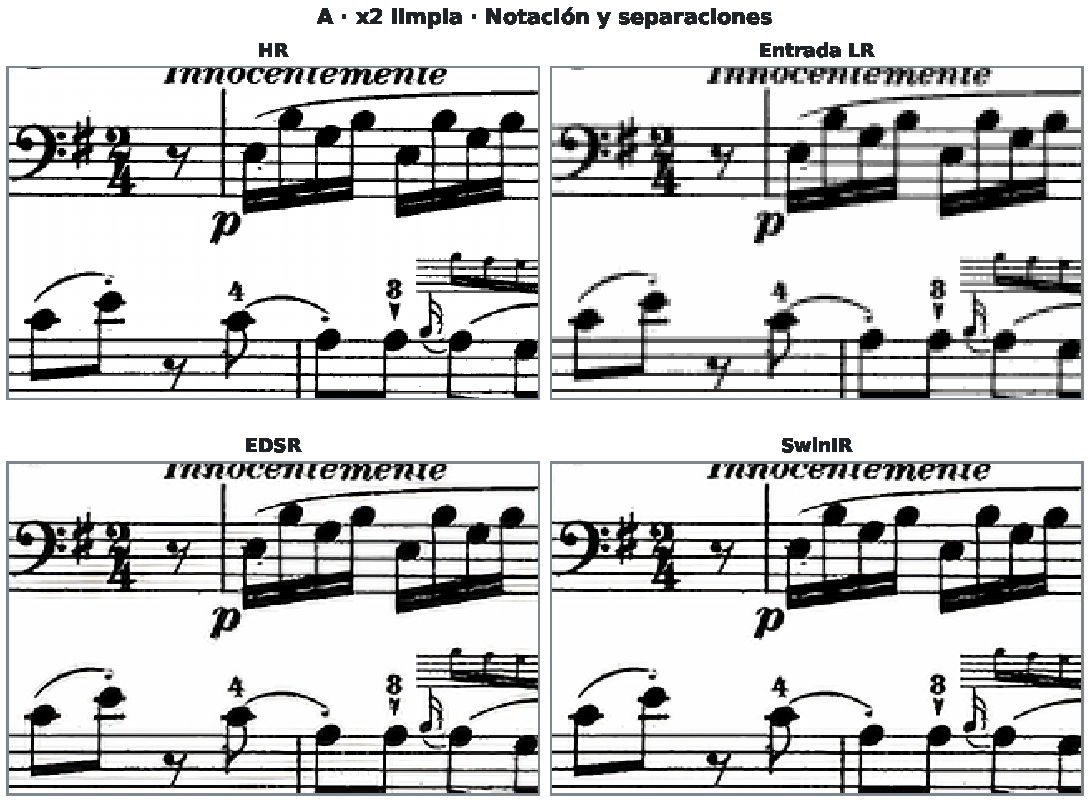
\includegraphics[page=1,width=\textwidth]{figures/results/pretrained-detail-gallery.pdf}
  \caption[Detalle de reconstrucciones favorables y artefactos preentrenados]{Ampliaciones
  emparejadas de tres casos SMB de la revisión fija, en tres láminas consecutivas. En esta primera
  lámina, A: \texttt{smb-test-000252}, x2 limpia,
  \texttt{haydn\_sonata53\_3}, de Joseph Haydn. B: \texttt{smb-test-000264}, x2 fuerte,
  \texttt{hummel\_prelude67\_04}, de Johann Nepomuk Hummel. C: \texttt{smb-test-000526}, x4 fuerte,
  \texttt{mozart\_sonata03\_2}, de Wolfgang Amadeus Mozart. La cercanía a HR debe juzgarse en los
  contornos, espacios y marcas pequeñas; una salida más nítida puede conservar o añadir defectos.
  Fuente: elaboración propia a partir de SMB \cite{smbDatasetCard}; coordenadas idénticas para
  todos los paneles de cada caso, sin realce adicional.}
  \label{fig:pretrained-details}
\end{figure}
\clearpage

\begin{figure}[p]
  \centering
  \includegraphics[page=2,width=\textwidth]{figures/results/pretrained-detail-gallery.pdf}
  \caption[B: x2 fuerte, Hummel]{Textura y contornos de HR, LR, EDSR y SwinIR en el caso fijo Hummel, ya identificado en la Figura~\ref{fig:pretrained-details}. Se conserva el mismo encuadre sin remuestrear los píxeles de las salidas. Fuente: SMB \cite{smbDatasetCard}.}
\end{figure}
\clearpage

\begin{figure}[p]
  \centering
  \includegraphics[page=3,width=\textwidth]{figures/results/pretrained-detail-gallery.pdf}
  \caption[C: x4 fuerte, Mozart]{Pérdida de trazos y texto en el caso fijo Mozart, identificado en la Figura~\ref{fig:pretrained-details}. La reconstrucción puede perfilar el trazo sin recuperar su geometría original. Fuente: SMB \cite{smbDatasetCard}.}
\end{figure}
\clearpage


La Tabla~\ref{tab:qualitative-origin} separa el origen observable del problema. \emph{No claro} no
significa que la salida sea perfecta, sino que no se identificó un defecto atribuible al método en
el caso. \emph{Introducido/amplificado} indica una diferencia problemática respecto de LR, mientras
que \emph{no recuperado} indica que el daño ya estaba presente en LR. La tabla evita sumar ambos
fenómenos como si fueran equivalentes.

\begin{table}[htbp]
  \centering
  \footnotesize
  \setlength{\tabcolsep}{3pt}
  \caption{Origen observable de las incidencias en los seis casos cualitativos fijos. Fuente:
  elaboración propia a partir de la revisión del estudiante.}
  \label{tab:qualitative-origin}
  \begin{tabular}{p{0.15\textwidth}p{0.24\textwidth}p{0.25\textwidth}p{0.25\textwidth}}
    \toprule
    Condición & Bicúbica & EDSR & SwinIR \\
    \midrule
    x2 limpia & No claro & No claro & No claro \\
    x2 moderada & No claro & No claro & No claro \\
    x2 fuerte & No claro; sin mejora apreciable & Introducido o amplificado & Introducido o amplificado \\
    x4 limpia & No claro; sin mejora apreciable & Introducido o amplificado & Introducido o amplificado \\
    x4 moderada & Introducido o amplificado & Introducido o amplificado & Introducido o amplificado \\
    x4 fuerte & Presente en LR y no recuperado & Introducido o amplificado sobre LR dañada & Introducido o amplificado sobre LR dañada \\
    \bottomrule
  \end{tabular}
\end{table}

No se marcó ningún \emph{cambio musicalmente plausible} como categoría separada, pero sí símbolos
alterados o perdidos en cuatro casos EDSR y tres SwinIR. Por ello, la ausencia de aquella etiqueta
no demuestra conservación semántica. La evidencia cualitativa contradice cualquier interpretación
según la cual una mejora promedio de PSNR o SSIM garantice que todos los elementos musicales se
reconstruyan correctamente.

Estos datos no permiten estimar sensibilidad, especificidad ni tasa de errores. La selección
determinista cubre condiciones, no tipos de símbolo, compositores, tipografías o severidades reales;
además, la revisión fue realizada por un único evaluador no ciego. Su fuerza reside en refutar una
interpretación demasiado amplia de las métricas y en documentar modos de fallo concretos, no en
probar que un método sea más seguro que otro en toda la población.

\clearpage
\section{Adaptación secundaria de EDSR}
La selección por validación produjo el punto de control del paso 1.500 para x2, con L1 RGB media
0,01409, y el del paso 2.500 para x4, con 0,03158. La Figura~\ref{fig:adaptation-checkpoints}
muestra que x2 dejó de mejorar de forma sostenida, mientras que x4 alcanzó su mínimo en el último
punto permitido. Por tanto, el resultado x4 describe el presupuesto congelado y podría subestimar
una mejora posterior; no se prolongó el entrenamiento después de observar la prueba.

\begin{figure}[htbp]
  \centering
  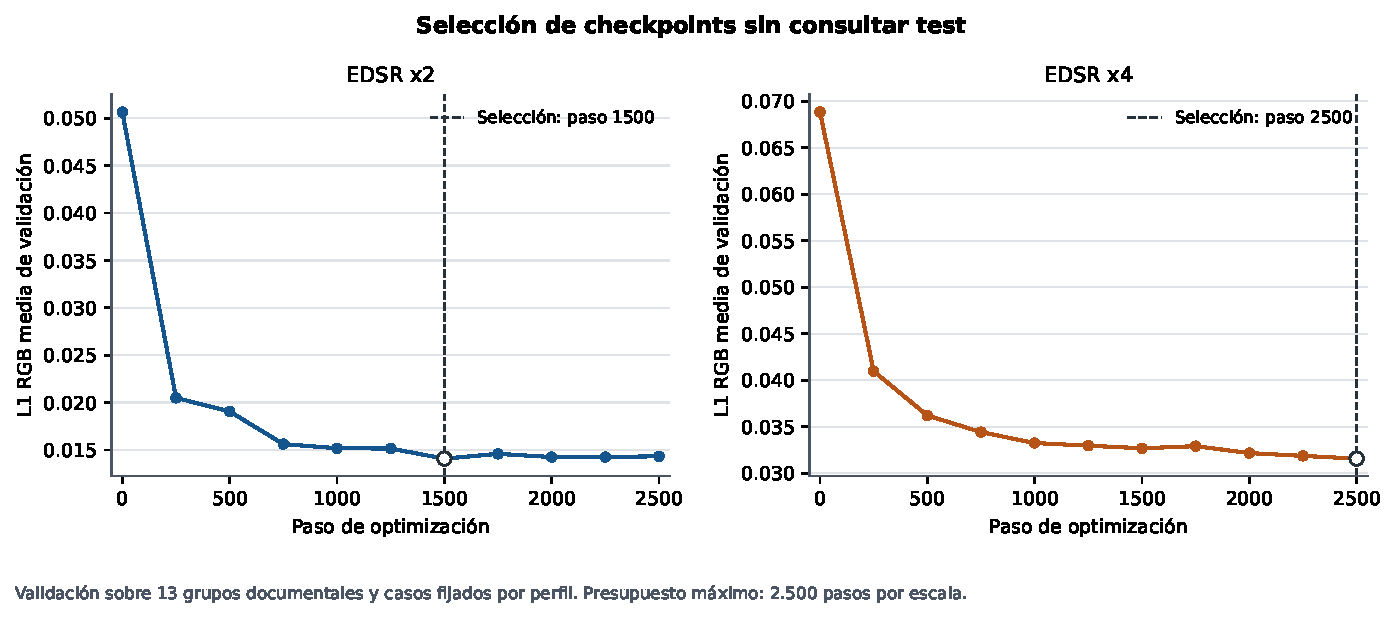
\includegraphics[width=\textwidth]{figures/results/adaptation-checkpoint-selection.pdf}
  \caption{Pérdida L1 RGB de validación y puntos de control elegidos para EDSR x2 y x4. La
  selección utiliza 13 grupos documentales y no consulta los 20 grupos documentales de prueba. Fuente:
  elaboración propia a partir del estudio de adaptación.}
  \label{fig:adaptation-checkpoints}
\end{figure}

El EDSR adaptado superó al EDSR oficial en PSNR-Y y SSIM-Y para las seis condiciones. Los doce
intervalos emparejados del 95\,\% quedaron por encima de cero. La ganancia PSNR-Y abarcó de
3,242 dB en x4 moderada a 7,844 dB en x2 fuerte; la ganancia SSIM-Y, de 0,0169 en x2 limpia a
0,1949 en x2 fuerte. En x2 mejoraron los 20 grupos documentales en ambas métricas. En x4, SSIM-Y mejoró en los
20; PSNR-Y lo hizo en 20 grupos bajo degradación limpia, 19 bajo moderada y 18 bajo fuerte.

\begin{table}[htbp]
  \centering
  \footnotesize
  \caption{Diferencia media emparejada EDSR adaptado menos EDSR oficial, con intervalo percentil
  del 95\,\% sobre 20 grupos documentales de prueba. Fuente: elaboración propia.}
  \label{tab:adaptation-deltas}
  \begin{tabular}{lrr}
    \toprule
    Condición & \(\Delta\) PSNR-Y (dB) & \(\Delta\) SSIM-Y \\
    \midrule
    x2 limpia   & 3,955 [3,492; 4,373] & 0,0169 [0,0143; 0,0200] \\
    x2 moderada & 4,719 [4,106; 5,336] & 0,0387 [0,0361; 0,0415] \\
    x2 fuerte   & 7,844 [7,328; 8,292] & 0,1949 [0,1786; 0,2104] \\
    x4 limpia   & 3,599 [2,978; 4,186] & 0,0602 [0,0487; 0,0722] \\
    x4 moderada & 3,242 [2,647; 3,771] & 0,0796 [0,0660; 0,0933] \\
    x4 fuerte   & 3,703 [2,723; 4,690] & 0,1558 [0,1365; 0,1746] \\
    \bottomrule
  \end{tabular}
\end{table}

La Figura~\ref{fig:adaptation-deltas} permite comparar magnitudes y denominadores sin mezclar este
estudio con los 64 grupos documentales del experimento principal. El modelo adaptado también superó a bicúbica
en ambas métricas y condiciones al nivel agregado. Sin embargo, las dos fuentes que empeoraron en
PSNR-Y frente al EDSR oficial bajo x4 fuerte fueron también las de menor separación de pentagrama
de la prueba. Es una observación \emph{post hoc} de solo dos casos, útil como hipótesis y no como
conclusión de subgrupo.
Los valores completos y sus intervalos se recogen en la Tabla~\ref{tab:adaptation-deltas}.

\begin{figure}[htbp]
  \centering
  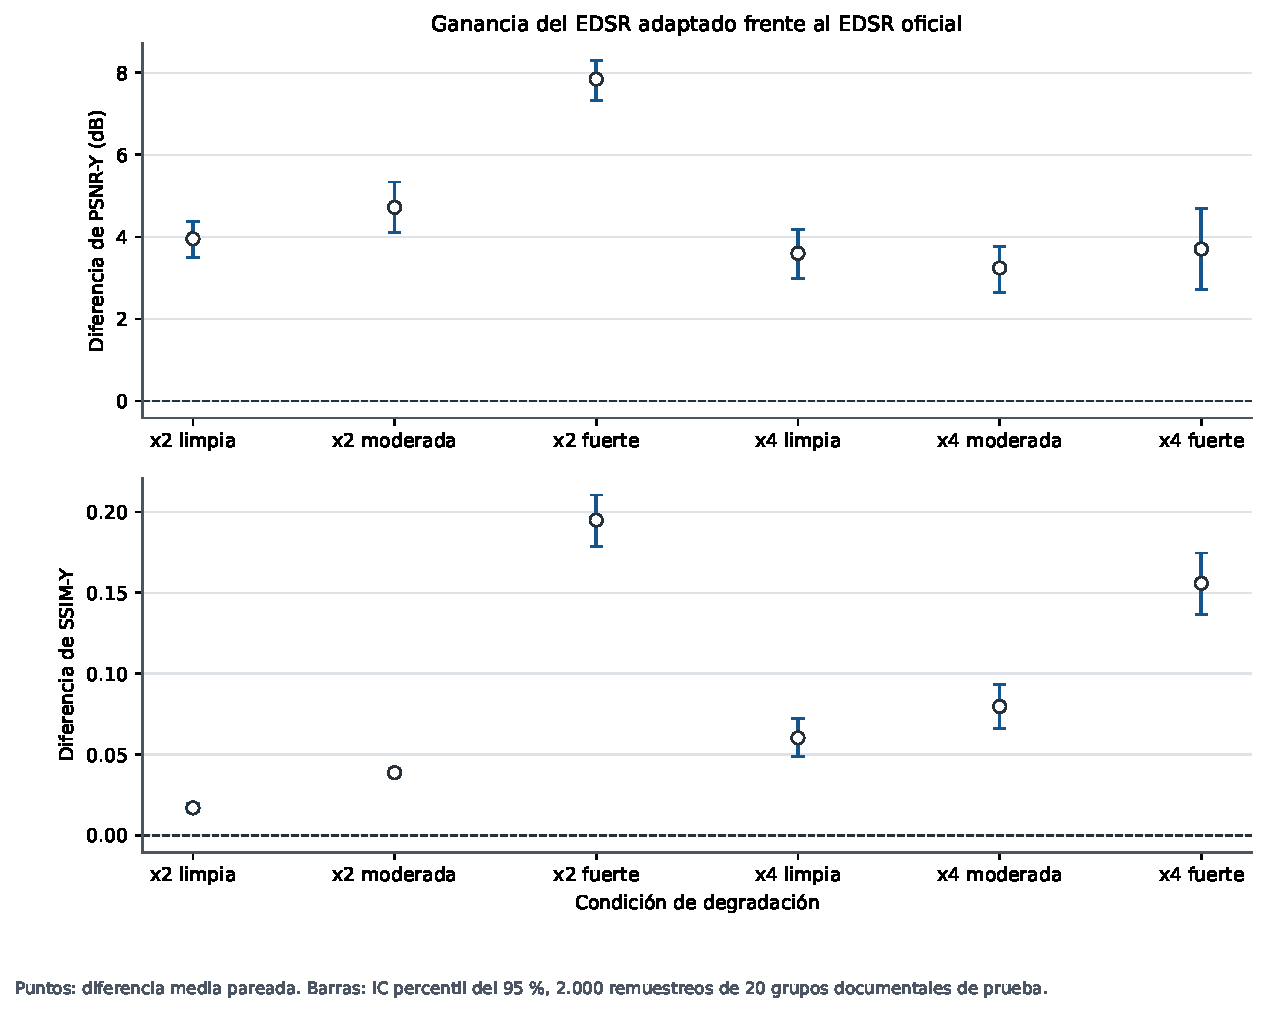
\includegraphics[width=0.92\textwidth]{figures/results/adaptation-deltas-vs-pretrained.pdf}
  \caption{Ganancia del EDSR adaptado respecto del EDSR oficial en 20 grupos documentales de prueba, con
  intervalos emparejados del 95\,\%. Fuente: elaboración propia a partir del estudio secundario.}
  \label{fig:adaptation-deltas}
\end{figure}

La revisión del estudiante clasificó los casos x2/x4 limpios y moderados como mejora sin defecto
nuevo claro, y los dos casos fuertes como daño ya presente en LR y no recuperado. Ninguno de los
seis se clasificó como daño introducido o amplificado por el EDSR adaptado. En los cuatro primeros,
el ajuste redujo halos y textura y definió mejor pentagramas y notación; persistieron limitaciones
menores en texto y en cabezas de nota muy próximas. En x2 fuerte, el mayor contraste no recuperó
alteraciones, ornamentos, líneas adicionales, texto ni dígitos pequeños. En x4 fuerte, el resultado
fue más legible que el EDSR oficial y reconstruyó mejor cabezas rellenas, plicas y ligaduras, pero
no recuperó digitaciones, símbolos pequeños, blancas ni texto. Podría servir para una consulta
aproximada, no para una interpretación musical final.

Las Figuras~\ref{fig:adapted-full-page}, \ref{fig:adapted-moderate}
y~\ref{fig:adapted-strong} muestran ambas caras del resultado con casos fijados antes de la
revisión. La primera conserva la página completa: permite verificar que el procesamiento mantiene
la disposición, los cinco sistemas, los márgenes y la densidad global, y muestra que el EDSR
adaptado se aproxima a la referencia con trazos más definidos que el oficial. Esta vista, sin
embargo, hace pequeños los detalles donde se decide la fidelidad musical; por eso se acompaña del
recorte alineado de la Figura~\ref{fig:adapted-moderate}. En \texttt{x4-moderate}, el ejemplo
\texttt{smb-test-000451} pasó de 23,184 a 26,684 dB de PSNR-Y y de 0,9254 a 0,9749 de SSIM-Y
entre el EDSR oficial y el adaptado. El recorte permite relacionar esa ganancia con menos halo,
trazos más rectos y una geometría más próxima a HR, sobre todo en pentagramas, ligaduras y
alteraciones. No equivale a afirmar que el modelo mejore todos los símbolos de la página.

\begin{figure}[p]
  \centering
  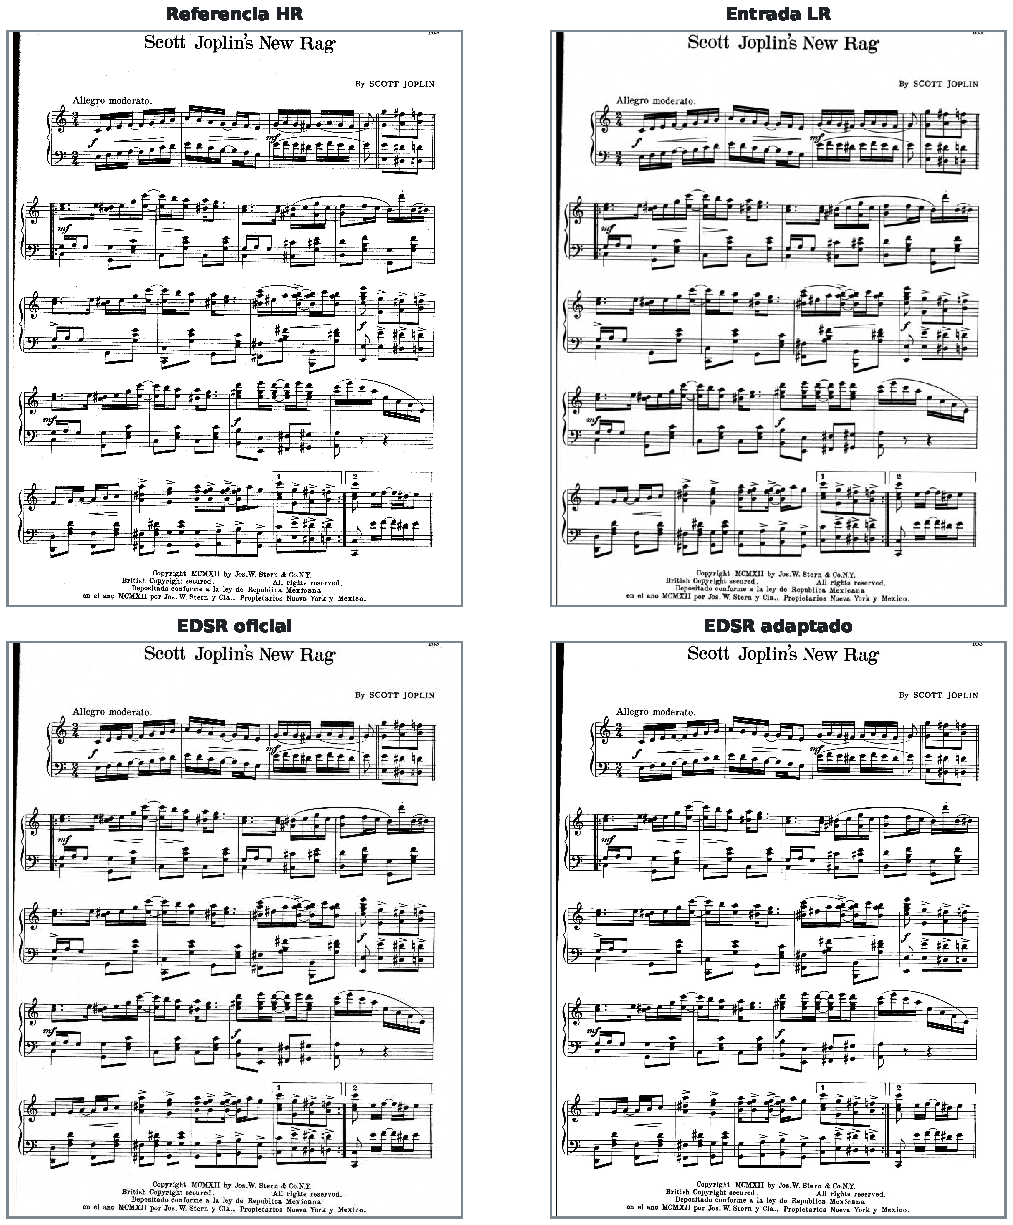
\includegraphics[width=\textwidth,height=0.82\textheight,keepaspectratio]{figures/results/adapted-full-page-x4-moderate.pdf}
  \caption[Comparación de página completa tras adaptar EDSR]{Comparación de página completa del
  caso fijo \texttt{smb-test-000451} bajo \texttt{x4-moderate}. La vista completa permite valorar
  estructura y legibilidad globales; los detalles se inspeccionan en la
  Figura~\ref{fig:adapted-moderate}. La LR está ampliada por vecino más próximo. Página de
  \emph{Scott Joplin's New Rag}, de Scott Joplin. Fuente: elaboración propia a partir de SMB,
  distribuido como CC BY-NC 4.0 \cite{smbDatasetCard,ccByNc40}; LR y reconstrucciones son
  transformaciones realizadas para este TFG.}
  \label{fig:adapted-full-page}
\end{figure}

\begin{figure}[htbp]
  \centering
  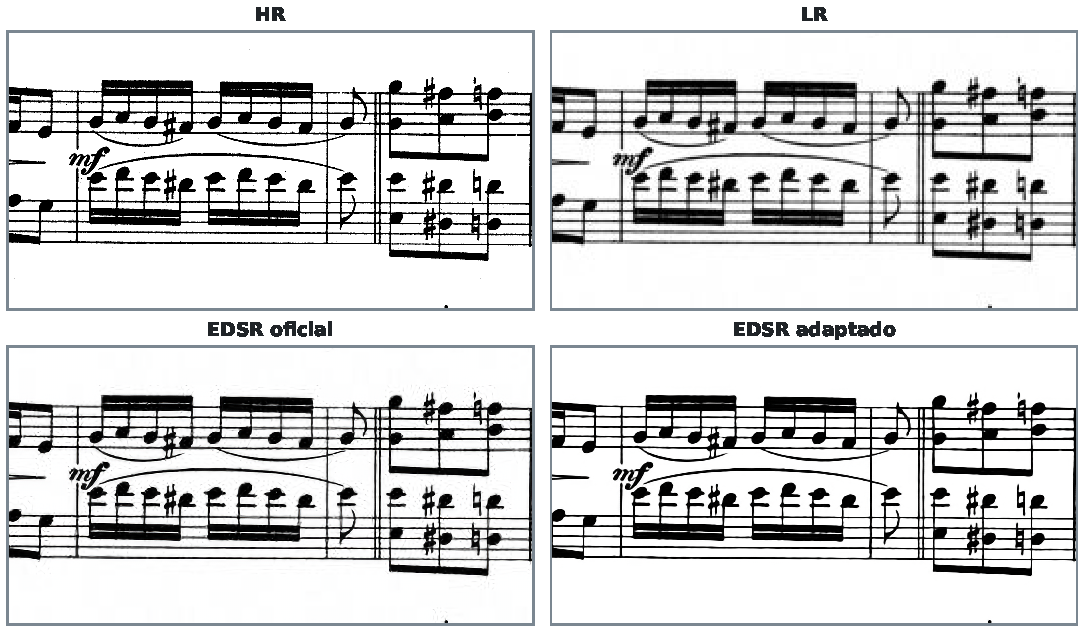
\includegraphics[width=\textwidth]{figures/results/adapted-comparison-x4-moderate.pdf}
  \caption[Mejora cualitativa del EDSR adaptado en x4 moderada]{Entrada y reconstrucciones del caso
  fijo \texttt{smb-test-000451} bajo degradación \texttt{x4-moderate}. La LR se amplía por vecino
  más próximo para visualizarla al tamaño HR. El EDSR adaptado reduce la textura y los halos del
  modelo oficial y aproxima mejor los trazos de la referencia. Fragmento de
  \emph{Scott Joplin's New Rag}, de Scott Joplin. Fuente: elaboración propia a partir de SMB
  \cite{smbDatasetCard}.}
  \label{fig:adapted-moderate}
\end{figure}

El caso \texttt{smb-test-000655}, en cambio, demuestra por qué una mejora métrica no autoriza una
promesa de restauración. Bajo \texttt{x4-strong}, el EDSR adaptado elevó PSNR-Y de 17,400 a
20,104 dB y SSIM-Y de 0,7860 a 0,9205 respecto del oficial, y eliminó gran parte de su textura
espuria. Aun así, la LR ya había perdido digitaciones, detalles internos y texto que el modelo no
podía deducir con fidelidad. En la Figura~\ref{fig:adapted-strong} el resultado adaptado es más
limpio, pero no es equivalente a la referencia ni apto para una edición musical final.

\begin{figure}[htbp]
  \centering
  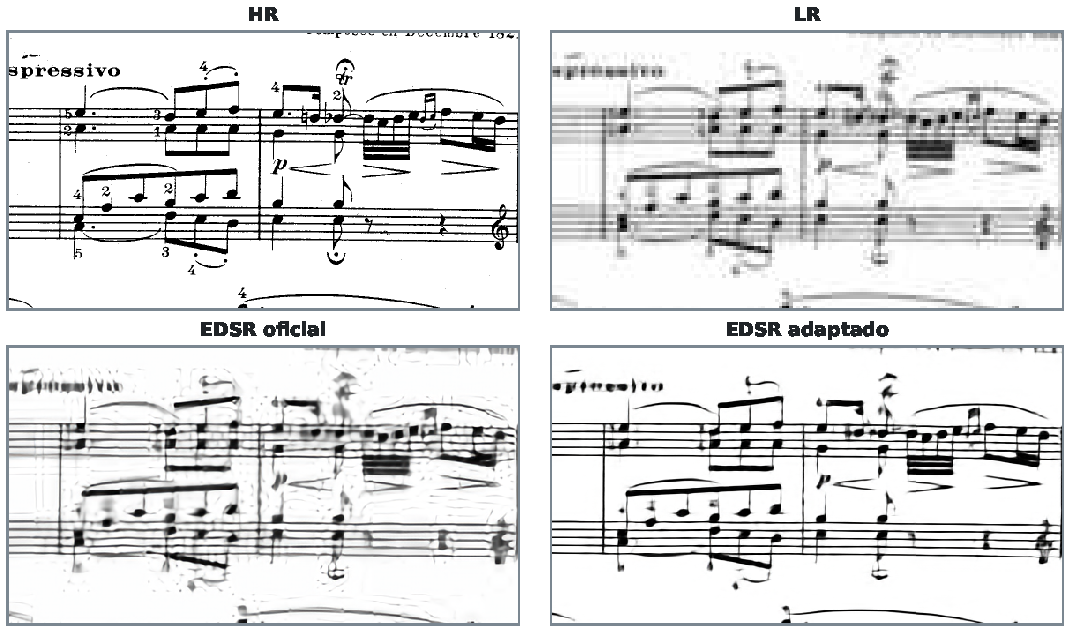
\includegraphics[width=\textwidth]{figures/results/adapted-limit-x4-strong.pdf}
  \caption[Límite del EDSR adaptado en x4 fuerte]{Caso fijo \texttt{smb-test-000655} bajo
  degradación \texttt{x4-strong}. La adaptación reduce los artefactos del EDSR oficial, pero no
  recupera toda la información ausente en LR; destacan la digitación y los signos pequeños. La LR
  se muestra ampliada por vecino más próximo. Fragmento de la Sonata para piano n.º 31, op.~110,
  de Ludwig van Beethoven, identificada como \texttt{beethoven\_sonata31\_1}. Fuente: elaboración
  propia a partir de SMB \cite{smbDatasetCard}.}
  \label{fig:adapted-strong}
\end{figure}

La Figura~\ref{fig:adapted-details} acerca ambos casos a detalles de tamaño comparable en el papel.
En A se pueden seguir las líneas y los límites de las alteraciones desde HR hasta el modelo
adaptado: la mejora consiste en aproximar la geometría de referencia, además de limpiar el fondo.
En B, las digitaciones y las marcas pequeñas permiten comprobar el límite: definir una mancha no
implica reconstruir el signo que ocupaba esa posición. Esta comparación ayuda a distinguir la
reducción de artefactos del EDSR oficial de la recuperación efectiva de información musical.

\begin{figure}[p]
  \centering
  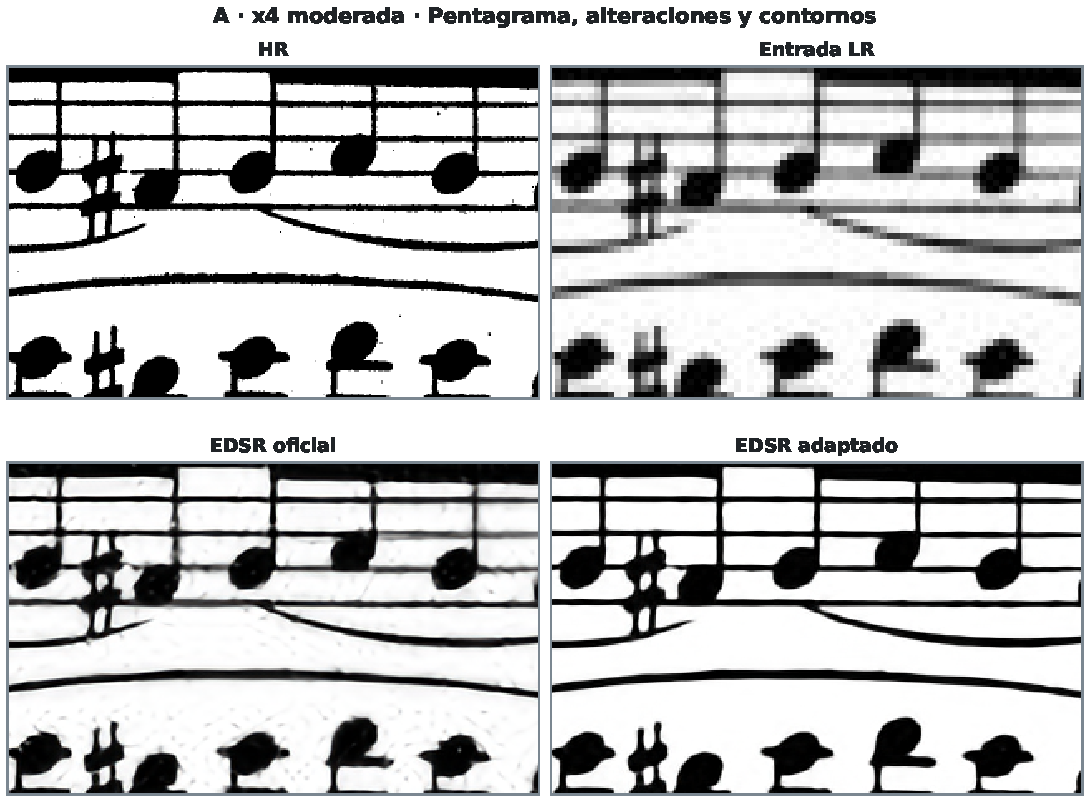
\includegraphics[page=1,width=\textwidth]{figures/results/adapted-detail-gallery.pdf}
  \caption[Detalle de la mejora y del límite del ajuste fino]{Las mismas regiones antes y después
  de adaptar EDSR, en dos láminas consecutivas. En esta primera, A, \emph{Scott Joplin's New Rag}, de Scott Joplin, caso
  \texttt{smb-test-000451} en x4 moderada; B, Sonata para piano n.º 31, op.~110, de Ludwig van
  Beethoven, caso \texttt{smb-test-000655} en x4 fuerte, en la siguiente lámina. El primer caso muestra la aproximación
  de los trazos a HR; el segundo conserva pérdidas visibles en elementos pequeños. Fuente:
  elaboración propia a partir de SMB \cite{smbDatasetCard}. Cada caso muestra el mismo recorte
  en HR, LR y ambas reconstrucciones, sin retoques de contraste ni limpieza posterior.}
  \label{fig:adapted-details}
\end{figure}
\clearpage

\begin{figure}[p]
  \centering
  \includegraphics[page=2,width=\textwidth]{figures/results/adapted-detail-gallery.pdf}
  \caption[B: límite de la adaptación, Beethoven]{Ampliación del caso Beethoven x4 fuerte, identificado en la Figura~\ref{fig:adapted-details}. El adaptado reduce artefactos, pero las digitaciones y marcas pequeñas de HR siguen sin reconstruirse con fidelidad. Fuente: SMB \cite{smbDatasetCard}.}
\end{figure}
\clearpage


Estos seis casos detectan límites, pero no permiten estimar su frecuencia ni demuestran corrección
semántica. En consecuencia, la adaptación respalda una mejora de fidelidad dentro de SMB y
degradaciones coincidentes, no una restauración musical autónoma.

\clearpage
\section{Transferencia externa y demostrador}
Al aplicar el EDSR adaptado sin reajuste a las doce obras externas, la diferencia media respecto al
EDSR oficial fue positiva en PSNR-Y y SSIM-Y en las seis condiciones
(Tabla~\ref{tab:external-deltas}). Los seis intervalos de PSNR-Y excluyeron cero; en SSIM-Y lo
hicieron cinco. La única comparación no resuelta fue x2 limpia, cuya media fue 0,0050 y cuyo
intervalo abarcó de -0,0014 a 0,0110. El resultado sostiene transferencia de fidelidad a otra
colección bajo el mismo generador sintético, sin demostrar recuperación de entradas LR naturales.

\begin{table}[htbp]
  \centering
  \footnotesize
  \caption{Diferencia media emparejada EDSR adaptado menos EDSR oficial en el corpus externo, con
  intervalo percentil del 95\,\% sobre doce obras. Fuente: elaboración propia.}
  \label{tab:external-deltas}
  \begin{tabular}{lrr}
    \toprule
    Condición & \(\Delta\) PSNR-Y (dB) & \(\Delta\) SSIM-Y \\
    \midrule
    x2 limpia   & 3,187 [1,193; 5,462] & 0,0050 [-0,0014; 0,0110] \\
    x2 moderada & 6,446 [5,299; 7,472] & 0,0287 [0,0248; 0,0340] \\
    x2 fuerte   & 8,204 [7,697; 8,724] & 0,1581 [0,1482; 0,1683] \\
    x4 limpia   & 2,440 [1,509; 3,418] & 0,0329 [0,0202; 0,0450] \\
    x4 moderada & 1,838 [0,990; 2,638] & 0,0433 [0,0319; 0,0553] \\
    x4 fuerte   & 2,376 [1,539; 3,242] & 0,0981 [0,0767; 0,1177] \\
    \bottomrule
  \end{tabular}
\end{table}

La revisión fija clasificó ocho casos como aceptables para consulta, tres como aceptables con
reservas y uno como rechazado. Los seis casos x2 fueron aceptados; en x4 limpia y moderada hubo un
aceptable y uno con reservas por condición; en x4 fuerte hubo uno con reservas y un rechazo. Este
último correspondió a una parte de percusión dispersa con cabezas y tipografía finas que no se
recuperaron de forma suficientemente consultable. En cinco casos no se observó defecto nuevo claro
y en siete el problema se atribuyó a información perdida en LR y no recuperada. Ninguno se marcó
como defecto introducido o amplificado, pero doce observaciones de un único revisor no demuestran
ausencia poblacional de ese riesgo.

\begin{figure}[htbp]
  \centering
  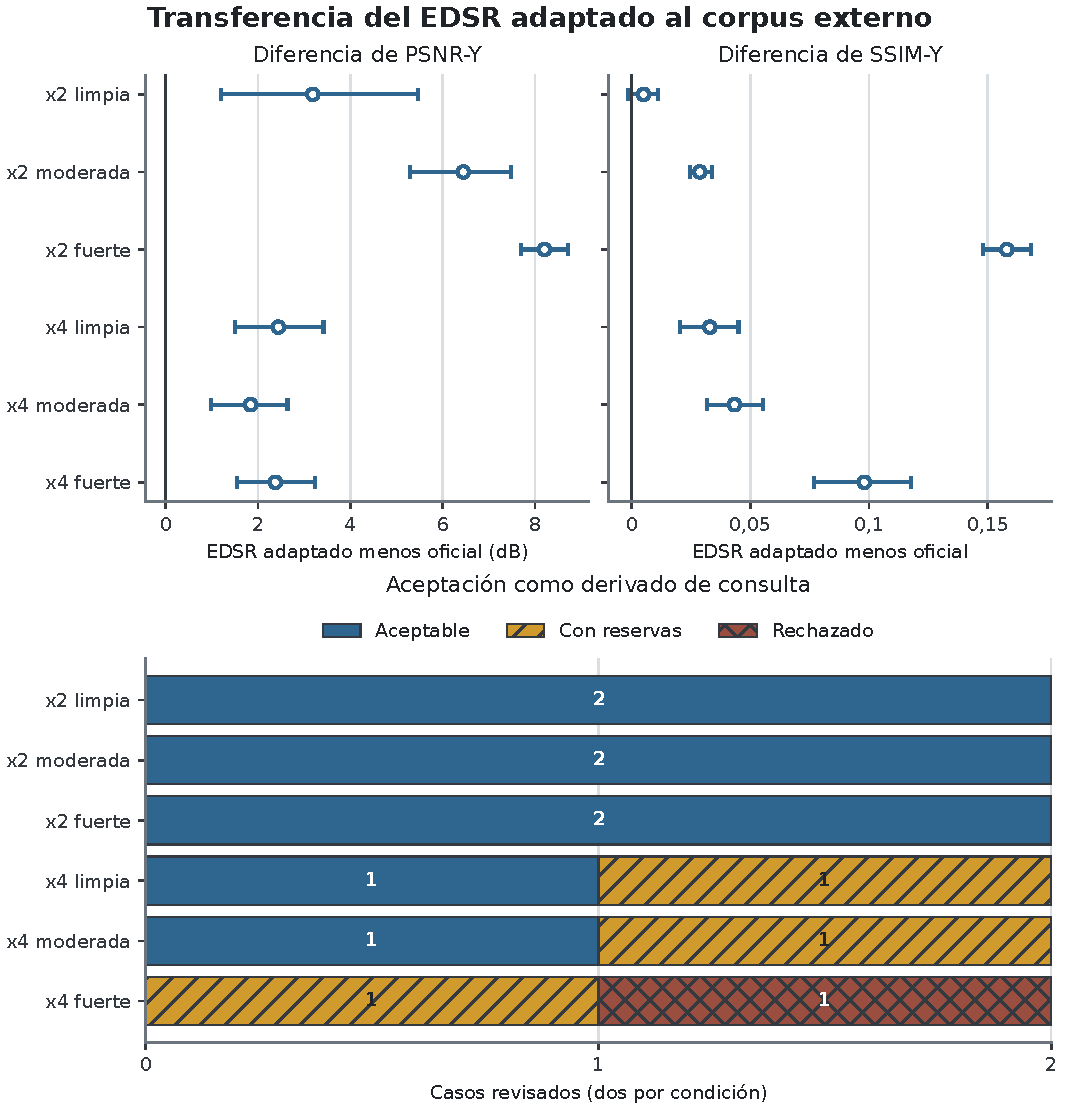
\includegraphics[width=0.98\textwidth]{figures/results/external-pilot-transfer.pdf}
  \caption[Transferencia y aceptación en el piloto externo]{Arriba, diferencia del EDSR adaptado
  respecto al oficial con intervalos emparejados del 95\,\% sobre doce obras externas. Abajo,
  decisiones del estudiante en los doce casos fijados, dos por condición. Los recuentos describen
  la muestra revisada y no son tasas de éxito. Fuente: elaboración propia.}
  \label{fig:external-pilot-transfer}
\end{figure}

La Figura~\ref{fig:external-pilot-transfer} muestra conjuntamente la transferencia cuantitativa y
las decisiones de consulta sin convertir estas últimas en una tasa poblacional. Las observaciones
convergieron en una limitación: el modelo adaptado redujo halos y textura y
definió mejor pentagramas y símbolos principales, pero el texto, los dígitos y la geometría fina
fueron los primeros elementos en no recuperarse al aumentar la degradación. En los dos escaneos HR
el revisor percibió incluso trazos más limpios, lo cual puede ser útil para consulta, pero no cambia
la condición del original como referencia documental ni prueba restauración histórica.

Las Figuras~\ref{fig:external-accepted} y~\ref{fig:external-rejected} hacen verificable esa síntesis
en el contexto completo de dos páginas que ya pertenecían al muestreo cualitativo fijo. No se
eligieron después por sus métricas: representan, respectivamente, un caso aceptado para consulta y
el único rechazo. Las otras diez comparaciones completas se reúnen en el
Anexo~\ref{app:external-case-atlas}; junto con estas dos, exponen visualmente las doce decisiones
sin omitir los casos con reservas. En \emph{Three Revelations from the Lotus Sutra}, la degradación x2 fuerte
difumina texto, alteraciones y trazos finos; el EDSR oficial mantiene un aspecto borroso, mientras
que el adaptado recupera contraste y continuidad suficientes para la consulta de la parte. No
reconstruye con exactitud todos los símbolos pequeños, por lo que la mejora visual no se traduce en
una garantía de identidad con HR.

\begin{figure}[p]
  \centering
  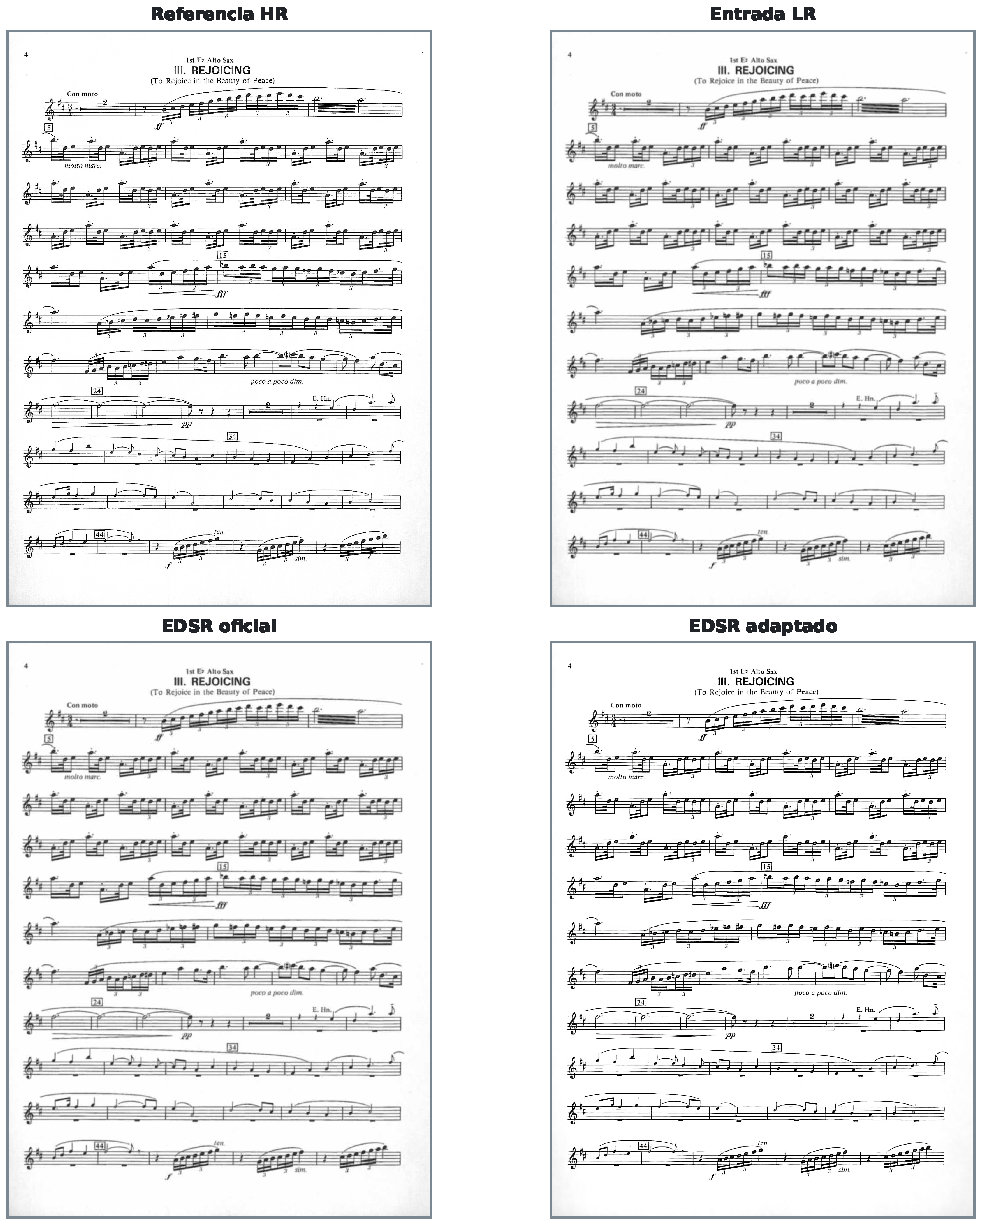
\includegraphics[width=\textwidth,height=0.82\textheight,keepaspectratio]{figures/results/external-accepted-full-page-x2-strong.pdf}
  \caption[Caso externo completo aceptado para consulta]{Caso externo fijo
  \texttt{three-revelations}, degradación \texttt{x2-strong}, aceptado para consulta. La salida
  adaptada mejora de forma visible la definición global frente al EDSR oficial, aunque texto y
  signos pequeños conservan daño procedente de LR. Extracto de una parte de saxofón alto primero en
  mi bemol de \emph{Three Revelations from the Lotus Sutra}, de Alfred Reed. Fuente: archivo musical
  de la Societat Joventut Musical d'Albal; página reproducida con autorización expresa para este
  TFG. La LR y las reconstrucciones son transformaciones de elaboración propia.}
  \label{fig:external-accepted}
\end{figure}

El rechazo \emph{Mari Carmen} aporta una condición documental distinta: notación de percusión
dispersa, cabezas no convencionales, tipografía fina y reducción x4 fuerte. El EDSR adaptado aumenta
el contraste respecto al oficial, pero no recompone con fiabilidad las cabezas, los matices y los
trazos más delgados. La baja densidad deja además pocos elementos redundantes que ayuden a
interpretar un símbolo degradado. Conservar este caso impide convertir once decisiones favorables
en una afirmación universal y fundamenta la vía profesional de rechazo del derivado.

\begin{figure}[p]
  \centering
  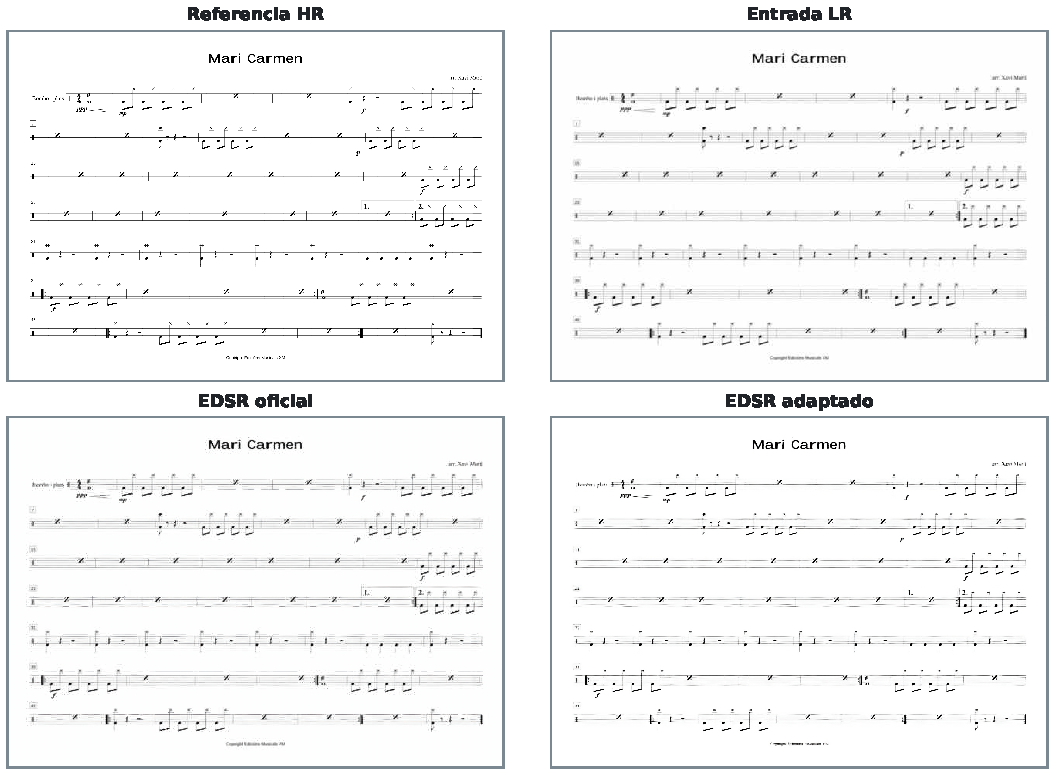
\includegraphics[width=\textwidth]{figures/results/external-rejected-full-page-x4-strong.pdf}
  \caption[Caso externo completo rechazado]{Caso externo fijo \texttt{mari-carmen}, degradación
  \texttt{x4-strong}, rechazado para consulta. El aumento de contraste del EDSR adaptado no recupera
  con suficiente fidelidad la notación fina de percusión perdida en LR. Extracto de la parte de
  bombo y platos de \emph{Mari Carmen}, arreglo de Xavi Martí. Fuente: archivo musical de la
  Societat Joventut Musical d'Albal; página reproducida con autorización expresa para este TFG. La
  LR y las reconstrucciones son transformaciones de elaboración propia.}
  \label{fig:external-rejected}
\end{figure}

La Figura~\ref{fig:external-details} permite inspeccionar tres situaciones de uso a mayor aumento:
una página aceptada, otra con reservas y la rechazada. En A se compara la limpieza de las notas
frente al EDSR oficial; en B, la separación entre los elementos sigue siendo una comprobación
necesaria aunque la página resulte globalmente consultable; en C, las cabezas y marcas finas de
percusión muestran por qué el aumento de contraste no basta: las cabezas en aspa de HR quedan
reducidas a manchas y no recuperan su geometría en las salidas. La decisión corresponde a la página
completa revisada, no solo al fragmento mostrado. Estos ejemplos complementan las doce páginas
completas e impiden confundir el aspecto de un detalle con una garantía de uso de toda la obra.

\begin{figure}[p]
  \centering
  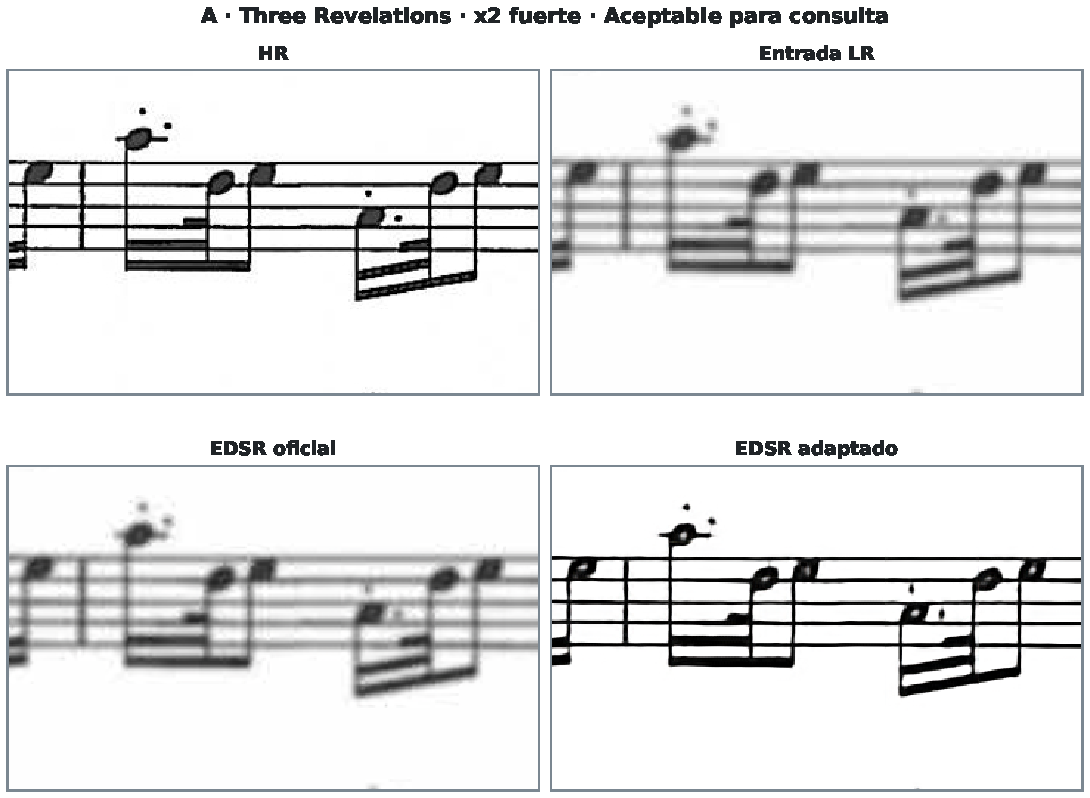
\includegraphics[page=1,width=\textwidth]{figures/results/external-detail-gallery.pdf}
  \caption[Ampliaciones de tres resultados del piloto externo]{Detalle de tres decisiones ya
  registradas, en tres láminas consecutivas. En esta primera, A: \emph{Three Revelations from the Lotus Sutra}, Alfred Reed, saxofón alto primero,
  x2 fuerte, aceptable para consulta. B: \emph{La rosa i el drac}, Francisco Valor, fliscorno
  segundo, x4 limpia, aceptable con reservas. C: \emph{Mari Carmen}, arreglo de Xavi Martí, bombo
  y platos, x4 fuerte, rechazado. Fuente: archivo musical de la SJMA; fragmentos reproducidos con
  autorización expresa para este TFG. LR y reconstrucciones son transformaciones propias;
  el encuadre se conserva dentro de cada caso y no se aplica realce adicional.}
  \label{fig:external-details}
\end{figure}
\clearpage

\begin{figure}[p]
  \centering
  \includegraphics[page=2,width=\textwidth]{figures/results/external-detail-gallery.pdf}
  \caption[B: caso externo con reservas]{Ampliación de La rosa i el drac, de Francisco Valor, fliscorno segundo, x4 limpia. La decisión de consulta con reservas corresponde a la página completa revisada. Fuente: archivo musical de la SJMA; reproducción autorizada para este TFG, con LR y reconstrucciones propias.}
\end{figure}
\clearpage

\begin{figure}[p]
  \centering
  \includegraphics[page=3,width=\textwidth]{figures/results/external-detail-gallery.pdf}
  \caption[C: caso externo rechazado]{Ampliación de Mari Carmen, arreglo de Xavi Martí, bombo y platos, x4 fuerte. Las cabezas en aspa de HR no recuperan su geometría. Fuente: archivo musical de la SJMA; reproducción autorizada para este TFG, con LR y reconstrucciones propias.}
\end{figure}
\clearpage


El demostrador local completó la carga validada de los dos puntos de control, el procesamiento por
teselas, la comparación original--derivado y la descarga PNG en sus pruebas automatizadas. En la
ejecución externa sobre CPU, la mediana por página fue de 25,8--26,4 segundos en x2 y de
10,3--10,6 en x4 para los dos EDSR. Esta inversión aparente se debe a que la entrada LR x2 contiene
más píxeles antes de reconstruir el mismo tamaño HR. El resultado es una prueba funcional local,
no una medición de usabilidad ni un servicio desplegado.

\clearpage
\section{Coste y comportamiento operativo}
La Figura~\ref{fig:runtime} resume la mediana por página en el dispositivo \texttt{cuda:0} de la
sesión Kaggle, que expuso dos Tesla T4 pero no ejecutó inferencia distribuida. Bicúbica
empleó entre 0,0038 y 0,0055 segundos; EDSR, entre 0,357 y 0,674; y SwinIR, entre 1,899 y 5,668.
SwinIR fue entre 5,2 y 8,5 veces más lento que EDSR y entre 486 y 1.045 veces más lento que
bicúbica, según la condición. Los tiempos \(\times 2\) fueron mayores porque la imagen de entrada
contiene más píxeles que en \(\times 4\) antes de reconstruir el mismo tamaño final.

A modo de escala operativa, procesar 1.000 páginas consecutivas bajo ese mismo entorno y sin contar
carga, descarga ni revisión supondría aproximadamente 4--6 segundos con bicúbica, 6--11 minutos con
EDSR y 32--95 minutos con SwinIR, según condición. Es una proyección aritmética del tiempo mediano,
no una prueba de rendimiento de un servicio: no incorpora concurrencia, memoria, colas ni
variabilidad entre documentos.

\begin{figure}[htbp]
  \centering
  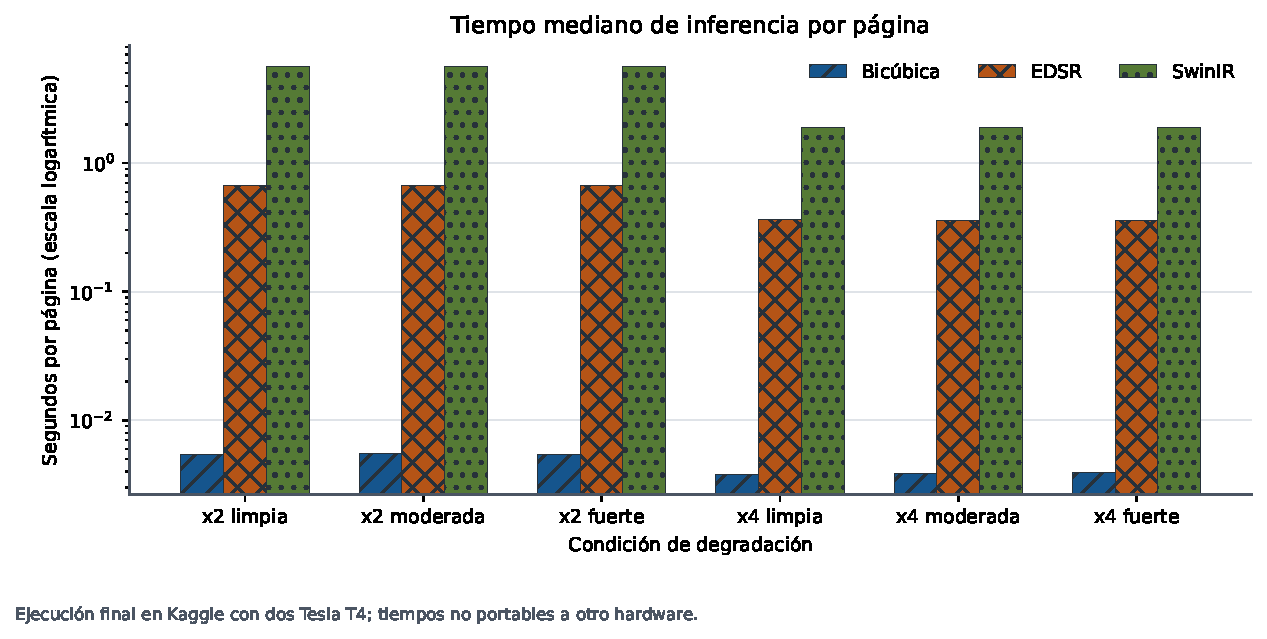
\includegraphics[width=\textwidth]{figures/results/runtime-median.pdf}
  \caption{Mediana del tiempo de reconstrucción por página en la ejecución Kaggle retenida. La
  escala vertical es logarítmica y los valores no se extrapolan a otro hardware. Fuente:
  elaboración propia.}
  \label{fig:runtime}
\end{figure}

El coste adicional de SwinIR solo queda justificado por fidelidad en las condiciones donde su
ventaja emparejada frente a EDSR fue clara. La ejecución no midió energía ni memoria máxima con una
instrumentación validada, por lo que no se atribuyen diferencias ambientales cuantitativas más
allá de hardware y duración.
